\subsection{Обратная связь по шифртексту}
\selectlanguage{russian}

\begin{figure}[bt]
	\centering
	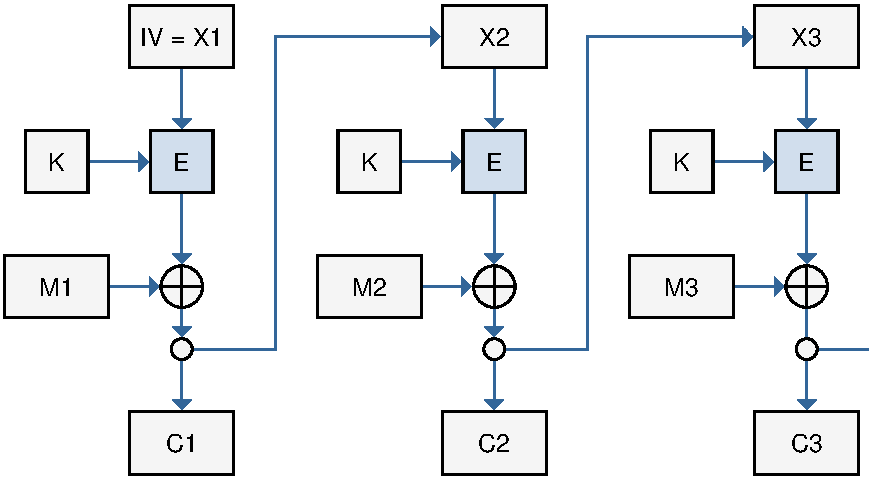
\includegraphics[width=1\textwidth]{pic/CFB}
	\caption{Режим обратной связи по шифртексту}
	\label{fig:CFB}
\end{figure}

В режиме обратной связи по шифртексту (\langen{Cipher FeedBack, CFB}, рис.~\ref{fig:CFB}) ключ $K_j$ получается с помощью процедуры шифрования предыдущего шифрованного блока $C_{j-1}$. Может быть использован не весь блок $C_{j-1}$, а только его часть. Как и в предыдущем случае, начальное значение ключа $K_0$ известно криптографу и легальному пользователю:
\[ \begin{array}{l}
    K_0 = \textrm{IV}, \\
    K_j = E_K(C_{j-1}), ~ j = 1, 2, \dots, n,\\
    C_j = K_j \oplus M_j.
\end{array} \]

У этого режима нет особых преимуществ по сравнению с другими режимами.
